\begin{frame}{Benchrmark Problems}
\begin{minipage}{.6\textwidth}
\begin{itemize}
    \item \small{Dataset in \textit{Zhang, EDBT 2004}: no longer available}
    \item \small{So we generate new benchmark problems:}
    \begin{itemize}
        \item \small{Extract the shape of all parks ($\approx 9000$) in Australia from \textit{OpenStreetMap}}
        \item \small{Use them as polygonal obstacles}
        \item \small{By normalizing their size and tiling them on empty square plane}
    \end{itemize}
\end{itemize}
\end{minipage}%
\begin{minipage}{.4\textwidth}
    \begin{adjustbox}{max totalsize={.9\textwidth}{.9\textheight}, right}
    \centering
    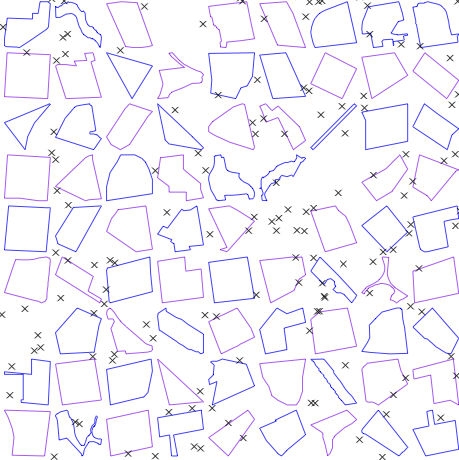
\includegraphics{pic/distribution.png}
    \end{adjustbox}
\end{minipage}
\end{frame}

\begin{frame}{Competitors}
\small{There are two types of test case:}
\begin{itemize}
    \item<1-> \small{Dense targets: $|T| \approx |O|$}
    \item<1-> \small{Sparse targets: $|T| <= 10, |O| \approx 9000$}
\end{itemize}
\small{In dense targets experiments, we compare between:}
\begin{itemize}
    \item<1-> \small{\textit{LVG} (from \textit{Zhang, EDBT 2004}}
    \item<1-> \small{Interval heuristic search}
    \item<1-> \small{Target heuristic search}
\end{itemize}
\small{In sparse targets experiments, we compare between:}
\begin{itemize}
    \item<1-> \small{burte-force Polyanya: run for all targets}
    \item<1-> \small{Interval heuristic search}
    \item<1-> \small{Target heuristic search}
\end{itemize}
\end{frame}

\begin{frame}{Dense targets}
\begin{minipage}{.5\textwidth}
    \centering
    \small{$|O| \approx 9000, |T| \approx |O|, k=1$}
    \begin{adjustbox}{max totalsize={.9\textwidth}{.9\textheight}, right}
    \centering
    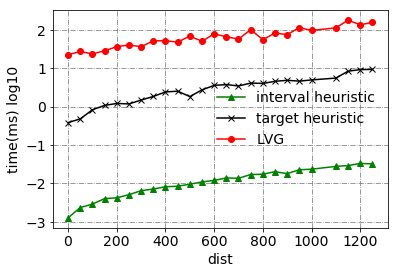
\includegraphics{pic/e1_dense_time.png}
    \end{adjustbox}
\end{minipage}%
\begin{minipage}{.5\textwidth}
    \centering
    \small{$|O| \approx 9000, |T| \approx |O|, k \in [1, 10]$}
    \begin{adjustbox}{max totalsize={.9\textwidth}{.9\textheight}, right}
    \centering
    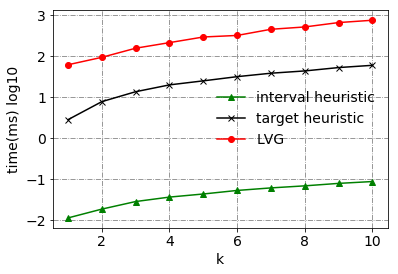
\includegraphics{pic/e2_dense_time.png}
    \end{adjustbox}
\end{minipage}
\begin{itemize}
    \item \small{\textit{Interval heuristic} is three order of magnitude faster than \textit{LVG}, in all aspects.}
\end{itemize}
\end{frame}

\begin{frame}{Sparse targets: fix $k=1$}
\centering
\small{$|O| \approx 9000, |T| \in [1, 10]$}
\begin{minipage}{.5\textwidth}
    \begin{adjustbox}{max totalsize={.9\textwidth}{.9\textheight}, right}
    \centering
    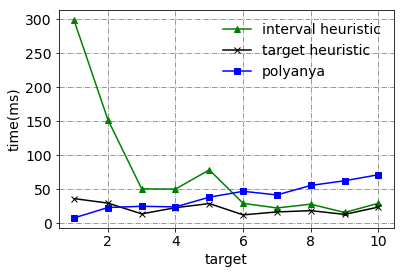
\includegraphics{pic/e3_time.png}
    \end{adjustbox}
\end{minipage}%
\begin{minipage}{.5\textwidth}
    \begin{adjustbox}{max totalsize={.9\textwidth}{.9\textheight}, right}
    \centering
    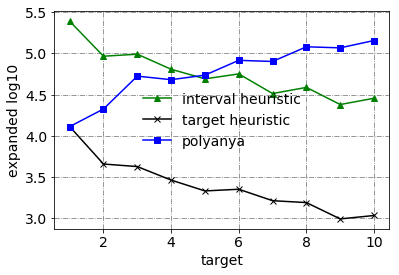
\includegraphics{pic/e3_gen.png}
    \end{adjustbox}
\end{minipage}
\begin{itemize}
    \item \small{\textit{Target heuristic} always has smaller search space. (right graph)}
    \item \small{It gradually lose such advantage when $|T|$ increase.}
    \item \small{Reason: the costly heuristic function.}
\end{itemize}
\end{frame}

\begin{frame}{Sparse targets: fix $|T|=10$}
\centering
\small{$|O| \approx 9000, k \in [1, 10]$}
\begin{minipage}{.5\textwidth}
    \begin{adjustbox}{max totalsize={.9\textwidth}{.9\textheight}, right}
    \centering
    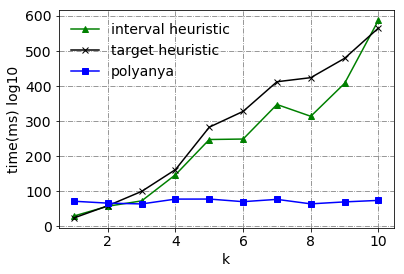
\includegraphics{pic/e2_sparse_time.png}
    \end{adjustbox}
\end{minipage}%
\begin{minipage}{.5\textwidth}
    \begin{adjustbox}{max totalsize={.9\textwidth}{.9\textheight}, right}
    \centering
    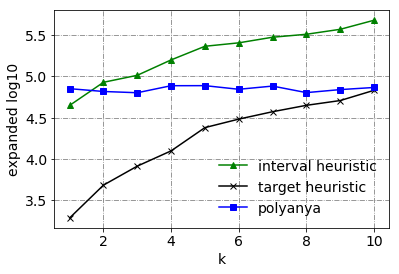
\includegraphics{pic/e2_sparse_gen.png}
    \end{adjustbox}
\end{minipage}
\begin{itemize}
    \item \small{\textit{Target heuristic} always faster than \textit{Interval heuristic}.}
    \item \small{It outcompeted by \textit{brute-force Polyanya} when $k>=2$.}
    \item \small{Reason: lazy reassignment becomes more frequent.}
\end{itemize}
\end{frame}